\subsection{Share of Detected Cases}
\label{subsec:data_share_known_cases}

 \comment[id=K]{Stoye called this the ascertainment rate if I remember right. Maybe we should replace this everywhere}

One important feature of our model is that we distinguish between undetected and detected
cases and that we model which cases are detected and which are not (see
Section~\ref{sub:testing} for a detailed description for how we model both rapid and PCR
tests). For our model it is important to have an estimate for the share of cases that is
detected in the absence of rapid tests ($\psi_t$). For this we rely on the
\cite[Dunkelzifferradar Project][]{Dunkelzifferradar2020} which uses estimates of the case
fatality rate to estimate the number of total cases given the number of CoViD-19 deaths
which are assumed to be perfectly observable. For 2020, we follow the reported share of
detected cases quite closely \textcolor{red}{only interpolating the phase of November
2020 where the testing policy was changed to give more priority to vulnerable groups
\citep{RKI2020a}. This lead to more tests being done among older age groups which are
also at the highest risk of dying from CoViD-19. We suspect that this led the estimated
share of detected cases to increase without a corresponding increase in the share of
detected cases in the overall population as PCR tests, a rare resource at the time, were
only moved to groups with a high case fatality ratio.}

% After Christmas 2020
Since vaccinations started after Christmas 2020 and these were predominantly given to
nursing homes in the beginning and other vulnerable groups in spring, we expect the
relationship between deaths and the number of total infections to change rapidly in 2021.
This is why we stop using the share of detected cases estimated by the Dunkelzifferradar
after Christmas. Instead, we assume that the share of detected cases would have stayed
the same in the absence of rapid tests. Thus, we also achieve in our model an increase in
the share of detected cases but this is driven from inside our model through increased
rapid testing which lead follow-up PCR tests when they are positive (see
Section~\ref{subsec:results_share_known_cases} and \ref{sub:testing}).

% Christmas and Easter
Lastly, we model reductions in the share known cases due to the two major holidays in our
simulation period, Christmas and Easter. During both holidays many laboratories did not
process tests and most physicians' offices were closed, leading to less PCR tests and
short and large drops in the share of known cases. The resulting share of detected cases
in the absence of rapid tests is shown in Figure~\ref{fig:share_known_cases_data}.

\begin{figure}[ht]
  \centering
  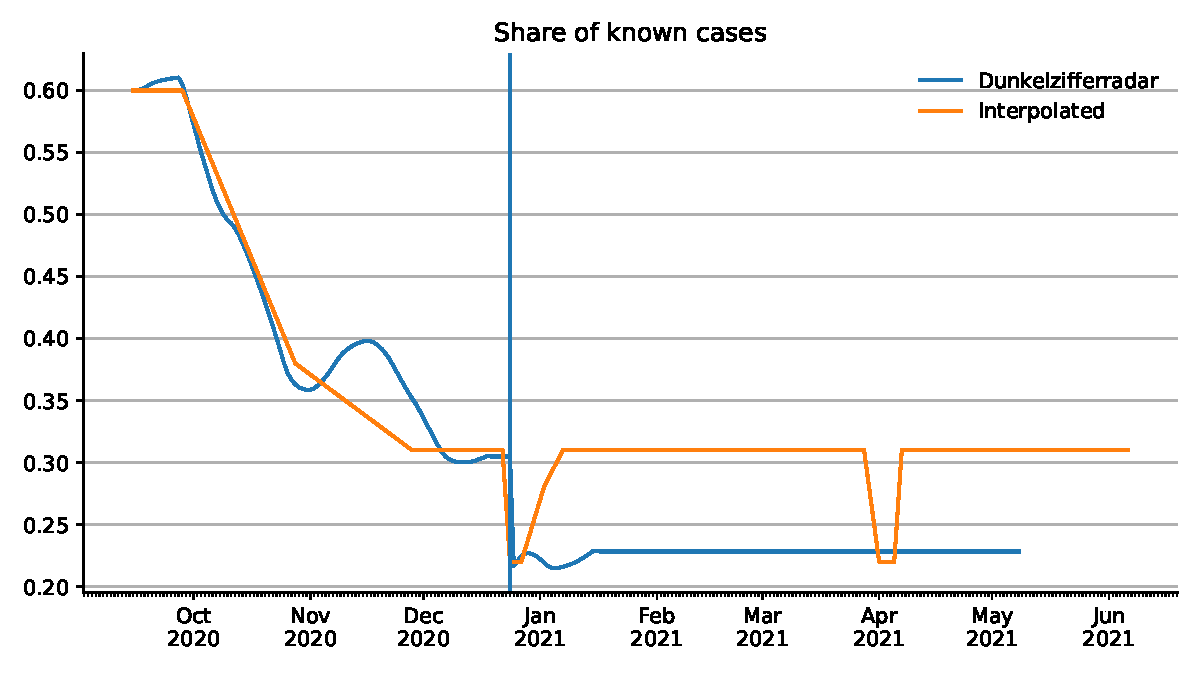
\includegraphics[width=0.5\textwidth]{figures/results/figures/data/testing/assumed_overall_share_known_cases}
  \caption{Share of Detected Cases in the Absence of Rapid Tests}
  \label{fig:share_known_cases_data}
  \floatfoot{\noindent \textit{Note:} The figure shows the share of cases that is
  reported as an official case via PCR confirmation. We use the overall share of known
  cases that was estimated through the case fatality ratio by the \cite[Dunkelzifferradar
  Project][]{Dunkelzifferradar2020} for all of 2020 and then assume it to be constant as
  vaccinations of the elderly strongly affect the case fatality rate which the project
  does not account for. Starting in 2021 in addition to the overall numbers of detected
  cases through symptoms and a random component, cases are also detected through
  confirmation of positive rapid tests which happens endogenously inside the model. For
  the public holidays of Christmas and Easter we lower the share of detected cases as
  fewer PCR tests are available during public holidays. See
  Figure~\ref{fig:share_known_cases_by_age_group} for how the share of detected cases
  develops in our model for each age group}.
\end{figure}

\FloatBarrier